% Example LaTeX document for GP111 - note % sign indicates a comment
\documentclass[12pt,a4paper,oneside]{article}
\usepackage{lmodern}
\usepackage[french]{babel}
\usepackage[T1]{fontenc}
\usepackage[utf8]{inputenc}
\usepackage{graphicx}
\usepackage{hyperref}
\usepackage{float}
\usepackage[backend=bibtex,style=verbose-trad2,natbib=true]{biblatex}


% Default margins are too wide all the way around. I reset them here
\setlength{\topmargin}{-.5in}
\setlength{\textheight}{9in}
\setlength{\oddsidemargin}{.125in}
\setlength{\textwidth}{6.25in}

\hypersetup{
    unicode=false,          % non-Latin characters in Acrobat’s bookmarks
    pdftoolbar=true,        % show Acrobat’s toolbar?
    pdfmenubar=true,        % show Acrobat’s menu?
    pdffitwindow=false,     % window fit to page when opened
    pdfnewwindow=true,      % links in new window
    colorlinks=true,       % false: boxed links; true: colored links
    linkcolor=black,          % color of internal links (change box color with linkbordercolor)
    citecolor=green,        % color of links to bibliography
    filecolor=magenta,      % color of file links
    urlcolor=cyan,          % color of external links
    linktoc=page
}

\begin{document}

\begin{titlepage}
\begin{flushright}
           
\includegraphics[scale=0.30]{../images/univorleans.png}\\ 
                      Département Informatique
\end{flushright}
\vspace{30mm}
\begin{center}
\textbf{\huge{Rapport SIG }}\\
\vspace{8mm}
\begin{large}
	\textit{Jordan FONTORBE}\\
	\textit{Willy FRANÇOIS}\\
	\textit{Jérémy MOROSI}\\
	\textit{Jean-Baptiste PERRIN}
\end{large}

\end{center}
\begin{figure}[b!]
\begin{flushright}
~~\\ ~~\\ ~~\\ ~~\\ ~~\\ ~~\\ ~~\\
\large{Année : 2013-2014}
\end{flushright}
\end{figure}
\end{titlepage}

\newpage

\tableofcontents
\newpage

\section{Introduction}

Dans le cadre de nos études, nous avions à réaliser un projet dans le domaine des Systèmes d'Information Géographique (SIG).

Ce projet est composé d'une application Android ainsi qu'un WebService.

L'application devait posséder 2 interfaces, une version local fonctionnant sans connexion internet, et une deuxième utilisant un WebService.

Le WebService devrait fournir un ensemble de service dont le fait de fournir un calcul d'itinéraire, ou la localisation.

\section{Répartition du travail}

\renewcommand{\labelitemi}{$\bullet$}
\begin{itemize}
\item Jean-Baptiste :
\begin{itemize}
\item Triangulation
\item Génération du graphe pour la version locale de l'application
\item Parsing du XML dans l'application (Graphe et voisins)
\item Calcul de l'itinéraire pour le WebService
\item WebService (AsyncTaskGetItineraire)
\end{itemize}

\item Jérémy :
\begin{itemize}
\item Partie OpenGL de l'application
\item Parsing du XML dans l'application (Affichage et arbre de décision)
\item Génération de l'arbre de décision pour la version locale de l'application
\item Architecture du code côté android (classes, découpage local/remote, interaction Activity/OpenGL)
\end{itemize}

\item Jordan :
\begin{itemize}
\item Structure de la base de données
\item Créations des tables SQL nécessaires pour la création de la carte
\item Modifications XML / modèle
\item Recherche des points proche d'un bâtiment
\item WebService (AsyncTaskGetLocation)
\end{itemize}

\item Willy :
\begin{itemize}
\item Structure de la base de données
\item Génération de la carte pour la version locale de l'application
\item Modifications XML / modèle
\item Recherche du bâtiment le plus proche pour le WebService
\item Mise en place du serveur WebService
\item WebService (AsyncTaskGetMap)
\end{itemize}
\end{itemize}




\begin{figure}[H]

\centering
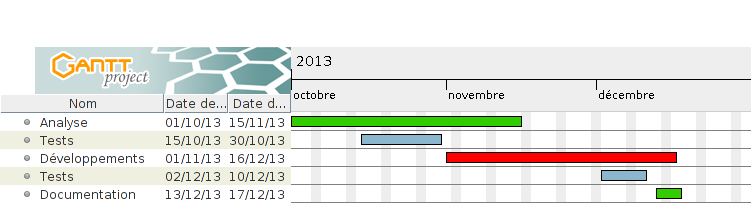
\includegraphics[width=1\textwidth]{../images/gantt.png}
\caption{Diagramme de GANTT}

\end{figure}

\section{Difficultés rencontrées}

Un problème s'est posé suite à l'import des données OpenStreetMap. En effet, nous avons remarqué que les coordonnées récupérées dans notre base de données ne ressemblaient pas à des latitudes et longitudes "normales". Nous avons compris alors que ces données étaient calculées avec le SRID 900913 alors que nous devions récupérer ces données avec le SRID 4326. Nous avons donc utilisé la fonction géométrique \texttt{ST\_Transform} pour corriger ce problème.\\

Nous avons rencontré des problèmes avec l'implémentation de l'algorithme du livre pour la génération de l'arbre de décision.
Comme solution, nous avons implémenté une version simplifiée, moins performante mais fonctionnelle,
décrite dans la documentation technique.


\section{Conclusion}

Au terme du délai qui nous était imparti, nous avons pu rendre une application permettant
d'afficher une carte de l'université d'Orléans issue de données OpenStreetMap et localisant
un bâtiment sélectionné sur l'écran pour la version locale.
Du côté de la version distante, nous récupérons et affichons la carte via le WebService.
Ce même WebService nous renvoi aussi un bâtiment en fonction d'une coordonnée GPS et
calcule un itinéraire entre deux bâtiments.

Cependant, nous n'avons pas été jusqu'à la localisation à l'intérieur des bâtiments.
En effet, n'ayant pas de données numériques décrivant les bâtiments,
il aurait fallu les créer manuellement et le temps ne nous le permettait pas.
\\

Ce projet nous a permis de mettre en pratique ce que nous avons vu en cours sur les systèmes
d'information géographique et sur quelques algorithmes géométriques.


\appendix
\end{document}
